\documentclass[aspectratio=169,xcolor={dvipsnames,table}]{beamer}
\usepackage[no-math,deluxe,haranoaji]{luatexja-preset}
\renewcommand{\kanjifamilydefault}{\gtdefault}
\renewcommand{\emph}[1]{{\upshape\bfseries #1}}
\usetheme{metropolis}
\metroset{block=fill}
\setbeamertemplate{navigation symbols}{}
\setbeamertemplate{blocks}[rounded][shadow=false]
\usecolortheme[rgb={0.7,0.2,0.2}]{structure}
%%%%%%%%%%%%%%%%%%%%%%%%%%
%% Change alert block colors
%%% 1- Block title (background and text)
\setbeamercolor{block title alerted}{fg=mDarkTeal, bg=mLightBrown!45!yellow!45}
\setbeamercolor{block title example}{fg=magenta!10!black, bg=mLightGreen!60}
%%% 2- Block body (background)
\setbeamercolor{block body alerted}{bg=mLightBrown!25}
\setbeamercolor{block body example}{bg=mLightGreen!15}
%%%%%%%%%%%%%%%%%%%%%%%%%%%
\usepackage[absolute,overlay]{textpos}
%\usepackage[grid=true,gridcolor=Maroon,subgridcolor=gray,gridunit=pt,texcoord]{eso-pic} %場所決めのためのgrid表示
%%%%%%%%%%%%%%%%%%%%%%%%%%%
%% さまざまなアイコン
%%%%%%%%%%%%%%%%%%%%%%%%%%%
%\usepackage{fontawesome}
\usepackage{fontawesome5}
\usepackage{figchild}
\usepackage{twemojis}
\usepackage{utfsym}
\usepackage{bclogo}
\usepackage{marvosym}
\usepackage{fontmfizz}
\usepackage{pifont}
\usepackage{phaistos}
\usepackage{worldflags}
\usepackage{jigsaw}
\usepackage{tikzlings}
\usepackage{tikzducks}
\usepackage{scsnowman}
\usepackage{epsdice}
\usepackage{halloweenmath}
\usepackage{svrsymbols}
\usepackage{countriesofeurope}
\usepackage{tipa}
%%%%%%%%%%%%%%%%%%%%%%%%%%%
\usepackage{tikz}
\usetikzlibrary{calc,patterns,decorations.pathmorphing,backgrounds}
\usepackage{tcolorbox}
\usepackage{tikzpeople}
\usepackage{circledsteps}
\usepackage{xcolor}
\usepackage{amsmath}
\usepackage{booktabs}
\usepackage{chronology}
\usepackage{signchart}
%%%%%%%%%%%%%%%%%%%%%%%%%%%
%% 場合分け
%%%%%%%%%%%%%%%%%%%%%%%%%%%
\usepackage{cases}
%%%%%%%%%%%%%%%%%%%%%%%%%%
\usepackage{pdfpages}
%%%%%%%%%%%%%%%%%%%%%%%%%%%
%% 音声リンク表示
\newcommand{\myaudio}[1]{\href{#1}{\faVolumeUp}}
%%%%%%%%%%%%%%%%%%%%%%%%%%
%% \myAnch{<名前>}{<色>}{<テキスト>}
%% 指定のテキストを指定の色の四角枠で囲み, 指定の名前をもつTikZの
%% ノードとして出力する. 図には remember picture 属性を付けている
%% ので外部から参照可能である.
\newcommand*{\myAnch}[3]{%
  \tikz[remember picture,baseline=(#1.base)]
    \node[draw,rectangle,line width=1pt,#2] (#1) {\normalcolor #3};
}
%%%%%%%%%%%%%%%%%%%%%%%%%%
%% \myEmph コマンドの定義
%%%%%%%%%%%%%%%%%%%%%%%%%%
%\newcommand{\myEmph}[3]{%
%    \textbf<#1>{\color<#1>{#2}{#3}}%
%}
\usepackage{xparse} % xparseパッケージの読み込み
\NewDocumentCommand{\myEmph}{O{} m m}{%
    \def\argOne{#1}%
    \ifx\argOne\empty
        \textbf{\color{#2}{#3}}% オプション引数が省略された場合
    \else
        \textbf<#1>{\color<#1>{#2}{#3}}% オプション引数が指定された場合
    \fi
}
%%%%%%%%%%%%%%%%%%%%%%%%%%%
%%%%%%%%%%%%%%%%%%%%%%%%%%%
%% 文末の上昇イントネーション記号 \myRisingPitch
%% 通常のイントネーション \myDownwardPitch
%% https://note.com/dan_oyama/n/n8be58e8797b2
%%%%%%%%%%%%%%%%%%%%%%%%%%%
\newcommand{\myRisingPitch}{
\begin{tikzpicture}[scale=0.3,baseline=0.3]
\draw[->,>=stealth] (0,0) to[bend right=45] (1,1);
\end{tikzpicture}
}
\newcommand{\myDownwardPitch}{
\begin{tikzpicture}[scale=0.3,baseline=0.3]
\draw[->,>=stealth] (0,1) to[bend left=45] (1,0);
\end{tikzpicture}
}
%%%%%%%%%%%%%%%%%%%%%%%%%%%%
%\AtBeginSection[%
%]{%
%  \begin{frame}[plain]\frametitle{授業の流れ}
%     \tableofcontents[currentsection]
%   \end{frame}%
%}

\usepackage{pxrubrica}
\UseTblrLibrary{counter}%%%%tabularrayとpauseが衝突することを回避する
\usepackage{lmodern}
%%%%%%%%%%%%%%%%%%%%%%%%%%%%%%%%%%%%%%%%%%
%%%%%%%%%%%%%%%%%%%%%%%%%%%
%%%%%%%%%%%%%%%%%%%%%%%%%%%
% --- Color Customization (Urban Night Theme) ---
% Deep Midnight Blue for background
\definecolor{CityNight}{HTML}{0B1021} 
% Vibrant Cyan for accents/structure% Vibrant Cyan for accents/structure
\definecolor{NeonCyan}{HTML}{00F0FF}
% Soft White for text
\definecolor{CloudWhite}{HTML}{F0F0F0}
% Muted gray for table rows
\definecolor{TableRowOdd}{HTML}{161B33}
\definecolor{TableRowEven}{HTML}{0B1021}

% --- Font Setup ---
% Metropolis uses Fira Sans by default if compiled with XeLaTeX/LuaLaTeX.
% Ensure fonts are readable.
\usefonttheme{professionalfonts}
%%%%%%%%%%%%%%%%%%%%%%%%%%
\title{English is fun.}
\subtitle{曜日、月、季節}
\author{}
\institute[]{}
\date[]

%%%%%%%%%%%%%%%%%%%%%%%%%%%%
%% TEXT
%%%%%%%%%%%%%%%%%%%%%%%%%%%%
\begin{document}

\begin{frame}[plain]
  \titlepage
\end{frame}

\section*{授業の流れ}
\begin{frame}[plain]
  \frametitle{授業の流れ}
  \tableofcontents
\end{frame}

\section{曜日}
%%%%%%%%%%%%%%%%%%%%%%%%%%%%%%%%%%%%%%%%%%%%%%%%%%
\begin{frame}[plain]{曜日}
\centering
\begin{tblr}{
  colspec = {rll}, 
%  column{2} = {fg=blue},   % 第7列の文字を青に
 row{odd} = {bg=azure8},
 row{1} = { bg=azure3, fg=white},
 row{2} = {fg=Maroon!80},    % 第2列の文字を赤に
 row{Z} = {fg=azure3},
 hline{Z} = {0.08em},    % \toprule, \midrule, \bottomrule
%  hline{3} = {0.5pt}       % もう1つの \midrule
 baseline=t,
 cell{1}{3} = {halign=r},
 cells={cmd=\onslide<\arabic{rownum}->} %%%%tabularrayとpauseが衝突することを回避する方法→https://github.com/lvjr/tabularray/issues/226
}
    & & {\scriptsize \myaudio{./audio/002_day_month_season_01.mp3}}\\
  日 & Sunday & \textipa{/s\'\textturnv nd\`eI/}\\
  月 & Monday & \textipa{/m\'\textturnv nd\`eI/}\\
  火 & Tuesday & \textipa{/t(j)\'u:zd\`eI/}\\ 
  水 & Wednesday & \textipa{/w\'enzd\`eI/}\\
  木 & Thursday & \textipa{/T\'\textrhookschwa :zd\`eI/}\\
  金 & Friday & \textipa{/fr\'aId\`eI/}\\
  土 & Saturday & \textipa{/s\'\ae t\textrhookschwa d\`eI/}\\
\end{tblr}
\end{frame}
%%%%%%%%%%%%%%%%%%%%%%%%%%%%%%%%%%%%%%%%%%%%%%%%%
\begin{frame}[plain]{曜日のたずね方など}
 
\Large

week \textipa{/w\'\i:k/} 週

\pause

\begin{enumerate}[<+->]
 \item What day of the week is it today? --- It's Friday.
 \item What day is it today? --- It's Saturday.
\end{enumerate}

\pause
\vspace{20pt}

weekday \textipa{/w\'\i:kd\`eI/} 週日\hspace{40pt}
\pause
weekend \textipa{/w\'\i:k\`end/} 週末

\pause

\begin{enumerate}[<+->]
\setcounter{enumi}{2}
 \item We work on \textbf{weekdays}.
 \item Have a nice \textbf{weekend}!
\end{enumerate}

\hfill{\scriptsize 0223\,\myaudio{./audio/002_day_month_season_011.mp3}}
\end{frame}
%%%%%%%%%%%%%%%%%%%%%%%%%%%%%%%%%%%%%%%%%%%%%%%%
\section{天体}
%%%%%%%%%%%%%%%%%%%%%%%%%%%%%%%%%%%%%%%%%%%%%%%%%
\begin{frame}[plain,t]{天体}
 \centering
\begin{tblr}{
        colspec = {lll},      % 2列とも中央揃え
        rowsep = 1.5pt,        % 行間の微調整(お好みで)
 cells={cmd=\onslide<\arabic{rownum}->} %%%%tabularrayとpauseが衝突することを回避する方法→https://github.com/lvjr/tabularray/issues/226
    }
        \toprule
        日本語名 & 英語名 \\
        \midrule
        太陽    & Sun \textipa{/s\'2n/}\\
        水星    & Mercury \textipa{/m\'\textrhookschwa :kjUri/}\\
        金星    & Venus \textipa{/v\'\i:n@s/}\\
        地球    & Earth \textipa{/\'\textrhookschwa :T/}&月 Moon \textipa{/m\'u:n/}\\
        火星    & Mars \textipa{/m\'A\textrhookschwa z/}\\
        木星    & Jupiter \textipa{/dZ\'u:p@t\textrhookschwa /}\\
        土星    & Saturn \textipa{/s\'\ae t\textrhookschwa n/}\\
        天王星  & Uranus \textipa{/j\'Ur@n@s/}\\
        海王星  & Neptune \textipa{/n\'ept(j)u:n/}\\
        \bottomrule
    \end{tblr}

\hfill{\scriptsize 0350\,\myaudio{./audio/002_day_month_season_planets.mp3}}

\end{frame}
%%%%%%%%%%%%%%%%%%%%%%%%%%%%%%%%%%%
\begin{frame}[plain]{How to Remember the Order of the Planets}
 
My Very Educated Mother Just Served Us Noodles.

わたしのとても教養のあるおかあさんが、たったいまわたしたちに麺を出してくれた
\end{frame}
%%%%%%%%%%%%%%%%%%%%%%%%%%%%%%%%%%
\begin{frame}[plain]
 
\includegraphics[width=1.01\textwidth]{./images/nanobanana-output/002_day_month_season_universe.png}
\begin{textblock*}{0.8\linewidth}(29pt,235pt)
\visible<2->{
\scalebox{1}{
\begin{tikzpicture}
  \node[fill=white] {the Solar System\hspace{12pt}My Very Educated Mother Just Served Us Noodles};
\end{tikzpicture}}
}
\end{textblock*}
\end{frame}
%%%%%%%%%%%%%%%%%%%
\begin{frame}[plain]{天体}
 \centering
\begin{tblr}{
        colspec = {lll},      % 2列とも中央揃え
        rowsep = 2pt,        % 行間の微調整(お好みで)
 cells={cmd=\onslide<\arabic{rownum}->} %%%%tabularrayとpauseが衝突することを回避する方法→https://github.com/lvjr/tabularray/issues/226
    }
        \toprule
        日本語名 & 英語名 \\
        \midrule
        宇宙(空間)    & space \textipa{/sp\'eIs/}\\
        宇宙(全体)    & universe \textipa{/j\'u:n@v\`\textrhookschwa :s/}\\
        恒星    & star \textipa{/st\'A\textrhookschwa /}\\
        惑星    & planet \textipa{/pl\'\ae nIt/}\\
        衛星    & satellite \textipa{/s\'\ae t@l\`aIt/}\\
        彗星    & comet \textipa{/k\'AmIt/}\\
        天の川  & the Milky Way \textipa{/D@ m\'Ilki w\'eI/}\\
        \bottomrule
    \end{tblr}

\hfill{\scriptsize 0251\,\myaudio{./audio/002_day_month_season_stars.mp3}}

\end{frame}
%%%%%%%%%%%%%%%%%%%%%%%%%%%%%%%%%%%%%%%%%%%%%%%%%%
%%%%%%%%%%%%%%%%%%%%%%%%%%%%%%%%%%%%%%%%%%%%%%%%%%
\section{month \textipa{/m\'\textturnv nT/}   season \textipa{/s\'\i:zn/}}
%%%%%%%%%%%%%%%%%%%%%%%%%%%%%%%%%%%%%%%%%%%%%%%%%%
\setbeamercolor{background canvas}{bg=}
\begin{frame}[plain]
\small

\begin{columns}
\begin{column}{.55\linewidth}
\begin{tblr}{
  colspec = {rlll}, 
%  column{2} = {fg=blue},   % 第7列の文字を青に
 row{1} = { bg=azure3, fg=white},
 row{2-3,13} = {bg=azure8},
 row{4-6} = {bg=SpringGreen!60},    
 row{7-9} = {bg=Goldenrod!60},    
 row{10-12} = {bg=Maroon!60!black!80, fg=white},
 column{4} = {bg=white},    
% row{Z} = {fg=azure3},
% hline{Z} = {0.08em},    % \toprule, \midrule, \bottomrule
%  hline{3} = {0.5pt}       % もう1つの \midrule
 baseline=t,
 cell{1}{3} = {halign=r},
 cells={cmd=\onslide<\arabic{rownum}->} %%%%tabularrayとpauseが衝突することを回避する方法→https://github.com/lvjr/tabularray/issues/226
}
    & month& {\scriptsize \textipa{/m\'\textturnv nT/}\hspace{15pt}\myaudio{./audio/002_day_month_season_02a.mp3}}\\
  1月 & January & \textipa{/dZ\'\ae nju\`eri/}&\myAnch{fuyu1}{white}{}\\
  2月 & February & \textipa{/f\'ebru\`eri/} \textipa{/f\'ebju\`eri/}\\
  3月 & March & \textipa{/m\'A\textrhookschwa tS/}\\ 
  4月 & April & \textipa{/\'eIpr@l/}&\myAnch{haru}{white}{}\\
  5月 & May & \textipa{/m\'eI/}\\
  6月 & June & \textipa{/dZ\'u:n/}\\
  7月 & July & \textipa{/dZUl\'aI/}&\myAnch{natsu}{white}{}\\
  8月 & August & \textipa{/\'O:g@st/}\\ 
  9月 & September & \textipa{/sept\'emb\textrhookschwa /}\\
  10月 & October & \textipa{/Akt\'oUb\textrhookschwa /}&\myAnch{aki}{white}{}\\
  11月 & November & \textipa{/nouv\'emb\textrhookschwa /}\\
  12月 & December & \textipa{/dIs\'emb\textrhookschwa /}&\myAnch{fuyu2}{white}{}\\
\end{tblr}
\end{column}
\begin{column}<14->{.4\linewidth}
\begin{tblr}{
  colspec = {lll}, 
%  column{2} = {fg=blue},   % 第7列の文字を青に
row{1} = { bg=azure3, fg=white},
 row{5} = {bg=azure8},
 row{2} = {bg=SpringGreen!60},    
 row{3} = {bg=Goldenrod!60},    
 row{4} = {bg=Maroon!60!black!80, fg=white},
column{1} = {bg=white},
  baseline=t,
 cells={cmd=\onslide<\arabic{rownum}->} %%%%tabularrayとpauseが衝突することを回避する方法→https://github.com/lvjr/tabularray/issues/226
}
    & \visible<14->{season}& {\scriptsize \textipa{/s\'\i:zn/}\hspace{27pt}\myaudio{./audio/002_day_month_season_02b.mp3}}\\
 \myAnch{spring}{white}{}&\visible<15->{spring}&\visible<15->{\textipa{/spr\'IN/}}\\
 \myAnch{summer}{white}{}&\visible<16->{summer}&\visible<16->{\textipa{/s\'\textturnv m\textrhookschwa /}}\\
 \myAnch{fall}{white}{}&\visible<17->{fall / autumn}&\visible<17->{\textipa{/f\'O:l/} \textipa{/\'O:t@m/}}\\
 \myAnch{winter}{white}{}&\visible<18->{winter}&\visible<18->{\textipa{/w\'Int\textrhookschwa/}}\\\
\end{tblr}
\end{column}
\end{columns}


\begin{tikzpicture}[remember picture,overlay]
 \onslide<15->{\draw[<-,line width=3pt,SpringGreen,opacity=.75] (haru.east) -- (spring.west);}
 \onslide<16->{\draw[<-,line width=3pt,Goldenrod,opacity=.75] (natsu.east) -- (summer.west);}
 {\onslide<17->\draw[<-,line width=3pt,Maroon,opacity=.75] (aki.east) -- (fall.west);}
 \onslide<18->{\draw[<-,line width=3pt,azure3,opacity=.75] (fuyu1.east) to[out=0,in=180] (winter.west);}
 \onslide<18->{\draw[<-,line width=3pt,azure3,opacity=.75] (fuyu2.315) to[out=0,in=200] (winter.west);}
\end{tikzpicture}

\end{frame}
%%%%%%%%%%%%%%%%%%%%%%%%%%%%%%%%%%%%%%%%%%%%%%%%%
\begin{frame}[plain]{Tips to Remember}
 \large
\begin{description}[        ]
 \item[1、2月] ---uary
 \item[6、7月] ju---
 \item[9, 10, 11, 12月] ---ber\\
10月以外は ---ember
\end{description}
\end{frame}
%%%%%%%%%%%%%%%%%%%%%%%%%%%%%%%%%%%%%%%%%%%%%%%%%%
\setbeamercolor{background canvas}{bg=}
\begin{frame}[plain]{date}
\centering
 \begin{tblr}{
%  colspec = {Q[r,1.1cm]Q[r,1.1cm]Q[r,1.1cm]Q[r,1.1cm]Q[r,1.1cm]Q[r,1cm]Q[r,1.1cm]}, % 
  colspec = {X[r]X[r]X[r]X[r]X[r]X[r]X[r]}, % 
  column{1} = {fg=red},          % 第1列の文字を赤に
  column{7} = {fg=blue},         % 第7列の文字を青に
  hline{1,2,Z} = {.08em},          % \toprule, \midrule, \bottomrule
  hline{3,4,5,6} = {0.05em}           % 追加した midrule
}
  Sun  & Mon & Tue & Wed & Thu & Fri & Sat \\
  \parbox[r]{\linewidth}{\raggedleft 1\\ \tiny first\\\mbox{}} &
\parbox[r]{\linewidth}{\raggedleft 2\\ \tiny second\\\mbox{}} &
\parbox[r]{\linewidth}{\raggedleft 3\\ \tiny third\\\mbox{}}  &
\parbox[r]{\linewidth}{\raggedleft 4\\ \tiny fourth\\\mbox{}}  &
\parbox[r]{\linewidth}{\raggedleft 5\\ \tiny fifth\\\mbox{}}  &
\parbox[r]{\linewidth}{\raggedleft 6\\ \tiny sixth\\\mbox{}}  &
\parbox[r]{\linewidth}{\raggedleft 7\\ \tiny seventh\\\mbox{}}  \\
\parbox[r]{\linewidth}{\raggedleft 8\\ \tiny eighth\\\mbox{}}&
\parbox[r]{\linewidth}{\raggedleft 9\\ \tiny ninth\\\mbox{}} &
\parbox[r]{\linewidth}{\raggedleft 10\\ \tiny tenth\\\mbox{}}& 
\parbox[r]{\linewidth}{\raggedleft 11\\ \tiny eleventh\\\mbox{}}   &
\parbox[r]{\linewidth}{\raggedleft 12\\ \tiny twelfth\\\mbox{}}  &
\parbox[r]{\linewidth}{\raggedleft 13\\ \tiny thirteenth\\\mbox{}}  &
\parbox[r]{\linewidth}{\raggedleft 14\\ \tiny fourteenth\\\mbox{}}  \\
\parbox[r]{\linewidth}{\raggedleft 15\\ \tiny fifteenth\\\mbox{}} &
\parbox[r]{\linewidth}{\raggedleft 16\\ \tiny sixteenth\\\mbox{}} &
\parbox[r]{\linewidth}{\raggedleft 17\\ \tiny seventeenth\\\mbox{}}  & 
\parbox[r]{\linewidth}{\raggedleft 18\\ \tiny eighteenth\\\mbox{}}  &
\parbox[r]{\linewidth}{\raggedleft 19\\ \tiny nineteenth\\\mbox{}}  & 
\parbox[r]{\linewidth}{\raggedleft 20\\ \tiny twentieth\\\mbox{}}  &
\parbox[r]{\linewidth}{\raggedleft 21\\ \tiny twenty-\\first}  \\
\parbox[r]{\linewidth}{\raggedleft 22\\ \tiny twenty-\\second} &
\parbox[r]{\linewidth}{\raggedleft 23\\ \tiny twenty-\\third} &
\parbox[r]{\linewidth}{\raggedleft 24\\ \tiny twenty-\\fourth}  & 
\parbox[r]{\linewidth}{\raggedleft 25\\ \tiny twenty-\\fifth}  &
\parbox[r]{\linewidth}{\raggedleft 26\\ \tiny twenty-\\sixth}  & 
\parbox[r]{\linewidth}{\raggedleft 27\\ \tiny twenty-\\seventh}  &
\parbox[r]{\linewidth}{\raggedleft 28\\ \tiny twenty-\\eighth}  \\
\parbox[r]{\linewidth}{\raggedleft 29\\ \tiny twenty-\\ninth}  &
\parbox[r]{\linewidth}{\raggedleft 30\\ \tiny thirtieth\\\mbox{}}  &
\parbox[r]{\linewidth}{\raggedleft 31\\ \tiny thirty-\\first}  &
\end{tblr}

\end{frame}
%%%%%%%%%%%%%%%%%%%%%%%%%%%%%%%%%%%%%%%%%%%%%%%%%%
\section{Date}
%%%%%%%%%%%%%%%%%%%%%%%%%%%%%%%%%%%%%%%%%%%%%%%%%%
\begin{frame}{Introduction}
    \begin{columns}
        \begin{column}{0.48\textwidth}
            \textbf{\textcolor{NavyBlue}{Cardinal Numbers}} \\
            (基数)
            \vspace{0.5em}
            \begin{itemize}
                \item "How many?"
                \item 数を数える時に使う
                \item 例: One, Two, Three
            \end{itemize}
        \end{column}
        \begin{column}{0.48\textwidth}
            \textbf{\textcolor{Maroon}{Ordinal Numbers}} \\
            (序数)
            \vspace{0.5em}
            \begin{itemize}
                \item "Which order?"
                \item 順序を表す時に使う
                \item 例: First, Second, Third
            \end{itemize}
        \end{column}
    \end{columns}
\end{frame}
%%%%%%%%%%%%%%%%%%%%%%%%%%%%%%%%%%%%%%%%%%%%%%%%%
% 3. Table 1-10
\begin{frame}[plain]{Numbers 1 - 10}
    \centering
    % tabularray settings for stylish look
    \begin{tblr}{
        colspec = {Q[c,m] Q[l,m] Q[l,m] Q[r,m]},
        width = 0.9\linewidth,
%        rows = {2.2em, m}, % Increase row height for readability
        row{odd} = {bg=NavyBlue!50},
%        row{odd} = {bg=TableRowOdd},
        row{even} = {bg=Yellow!50},
%        row{even} = {bg=TableRowEven},
        row{1} = {bg=CityNight!50, fg=white, font=\bfseries}, % Header
        hlines = {0.5pt, fg=gray!30},
        vlines = {0pt}, % Remove vertical lines for cleaner look
  cells={cmd=\onslide<\arabic{rownum}->} %%%%tabularrayとpauseが衝突することを回避する方法→https://github.com/lvjr/tabularray/issues/226
   }
        \# & Cardinal (基数) & Ordinal (序数) \\
        1 & one & \textbf{first} &(1st) \\
        2 & two & \textbf{second} &(2nd) \\
        3 & three & \textbf{third} &(3rd) \\
        4 & four & fourth &(4th) \\
        5 & five & \textbf{fifth} &(5th) \\
        6 & six & sixth &(6th) \\
        7 & seven & seventh &(7th) \\
        8 & eight & \textbf{eighth} &(8th) \\
        9 & nine & \textbf{ninth} &(9th) \\
        10 & ten & tenth &(10th) 
    \end{tblr}
\mbox{}\hfill{\tiny 0051}\,{\scriptsize \myaudio{../1st_grader/audio/014_when_07.mp3}}

\end{frame}
%%%%%%%%%%%%%%%%%%%%%%%%%%%%%%%%%%%%%%%%%%%%%%%%%
\begin{frame}[plain]{序数のつくりかたの原則}
 
\begin{description}
 \item<2->[日本語] 数字 $+$ 番目
 \item<3->[英語] 数字 $+$ th 
\end{description}

\vspace{30pt}

\hfill\visible<4->{ただし、例外に注意しましょう}

\hfill\visible<5->{例外となる場合は、\textbf{太い文字}で表示します}
\end{frame}
%%%%%%%%%%%%%%%%%%%%%%%%%%%%%%%%%%%%%%%%%%%%%%%%%%
\begin{frame}[plain]{Numbers 11 - 20}
    \centering
    \begin{tblr}{
        colspec = {Q[c,m] Q[l,m] Q[l,m] Q[r,m]},
        width = 0.9\linewidth,
%        rows = {2.2em, m},
        row{odd} = {bg=NavyBlue!50},
        row{even} = {bg=Yellow!50},
        row{1} = {bg=CityNight!50, fg=white, font=\bfseries},
        hlines = {0.5pt, fg=gray!30},
 cells={cmd=\onslide<\arabic{rownum}->} %%%%tabularrayとpauseが衝突することを回避する方法→https://github.com/lvjr/tabularray/issues/226
    }
        \# & Cardinal (基数) & Ordinal (序数) \\
        11 & eleven & eleventh &(11th) \\
        12 & twelve & \textbf{twelfth} &(12th) \\
        13 & thirteen & thirteenth &(13th) \\
        14 & fourteen & fourteenth &(14th) \\
        15 & fifteen & fifteenth &(15th) \\
        16 & sixteen & sixteenth &(16th) \\
        17 & seventeen & seventeenth &(17th) \\
        18 & eighteen & eighteenth &(18th) \\
        19 & nineteen & nineteenth &(19th) \\
        20 & twenty & \textbf{twentieth} &(20th) 
    \end{tblr}
\mbox{}\hfill{\tiny 0055}\,{\scriptsize \myaudio{../1st_grader/audio/014_when_08.mp3}}

\end{frame}
%%%%%%%%%%%%%%%%%%%%%%%%%%%%%%%%%%%%%%%%%%%%%%%%
\begin{frame}[plain]{Numbers 21 - 30}
    \centering
    % Showing the rule for compound numbers and tens
    \begin{tblr}{
        colspec = {Q[r,m] Q[l,m] Q[l,m] Q[r,m]},
        width = 0.95\linewidth,
 %       rows = {2.5em, m},
        row{odd} = {bg=NavyBlue!50},
        row{even} = {bg=Yellow!50},
        row{1} = {bg=CityNight!50, fg=white, font=\bfseries},
        hlines = {0.5pt, fg=gray!30},
 cells={cmd=\onslide<\arabic{rownum}->} %%%%tabularrayとpauseが衝突することを回避する方法→https://github.com/lvjr/tabularray/issues/226
    }
        \# & Cardinal (基数) & Ordinal (序数) \\
        21 & twenty-one & twenty-\textbf{first} &(21st) \\
        22 & twenty-two & twenty-\textbf{second} &(22nd) \\
        23 & twenty-three &twenty-\textbf{third} &(23rd)\\
        24 & twenty-four &twenty-fourth &(24th)\\
        25 & twenty-five &twenty-\textbf{fifth} &(25th)\\
        26 & twenty-six &twenty-sixth &(26th)\\
        27 & twenty-seven&twenty-seventh &(27th)\\
        28 & twenty-eight&twenty-\textbf{eighth} &(28th)\\
        29 & twenty-nine &twenty-\textbf{ninth} &(29th)\\
        30 & thirty & \textbf{thirtieth} &(30th) \\
    \end{tblr}
\mbox{}\hfill{\tiny 0058}\,{\scriptsize \myaudio{../1st_grader/audio/014_when_09.mp3}}


    \vspace{1em}

\raggedleft
    \small {Rule:} 20, 30 \ldots 90番目\hspace{1em} y $\to$ ie + th
\end{frame}
%%%%%%%%%%%%%%%%%%%%%%%%%%%%%%%%%%%%%%%%%%%%%%%%%
%%%%%%%%%%%%%%%%%%%%%%%%%%%%%%%%%%%%%%%%%%%%%%%%
\begin{frame}[plain]{Patterns 30 - 1000}
    \centering
    % Showing the rule for compound numbers and tens
    \begin{tblr}{
        colspec = {Q[r,m] Q[l,m] Q[l,m] Q[r,m]},
        width = 0.95\linewidth,
 %       rows = {2.5em, m},
        row{odd} = {bg=NavyBlue!40},
        row{even} = {bg=Yellow!50},
        row{1} = {bg=CityNight!50, fg=white, font=\bfseries},
        hlines = {0.5pt, fg=gray!30},
 cells={cmd=\onslide<\arabic{rownum}->} %%%%tabularrayとpauseが衝突することを回避する方法→https://github.com/lvjr/tabularray/issues/226
    }
        \# & Cardinal (基数) & Ordinal (序数) \\
        30 & thirty & thirtieth &(30th) \\
        40 & forty & fortieth &(40th) \\
        50 & fifty & fiftieth &(50th) \\
        60 & sixty & sixtieth &(60th) \\
        70 & seventy & seventieth &(70th) \\
        80 & eighty & eightieth &(80th) \\
        90 & ninety & ninetieth &(90th)\\
        100 & one hundred & one hundredth &(100th)\\
        1000 & one thousand & one thousandth &(1000th)
    \end{tblr}
\mbox{}\hfill{\tiny 0050}\,{\scriptsize \myaudio{../1st_grader/audio/014_when_10.mp3}}

\raggedleft
    \small {Rule:} 20, 30 \ldots\,\,90番目\hspace{1em} ty $\to$ tie $+$ th
\end{frame}
%%%%%%%%%%%%%%%%%%%%%%%%%%%%%%%%%%%%%%%%%%%%%%%%%
%%%%%%%%%%%%%%%%%%%%%%%%%%%%%%%%%%%%%%%%%%%%%%%
\setbeamercolor{background canvas}{bg=}
\begin{frame}[plain]{date}
\centering
 \begin{tblr}{
%  colspec = {Q[r,1.1cm]Q[r,1.1cm]Q[r,1.1cm]Q[r,1.1cm]Q[r,1.1cm]Q[r,1cm]Q[r,1.1cm]}, % 
  colspec = {X[r]X[r]X[r]X[r]X[r]X[r]X[r]}, % 
  column{1} = {fg=red},          % 第1列の文字を赤に
  column{7} = {fg=blue},         % 第7列の文字を青に
  hline{1,2,Z} = {.08em},          % \toprule, \midrule, \bottomrule
  hline{3,4,5,6} = {0.05em}           % 追加した midrule
}
  Sun  & Mon & Tue & Wed & Thu & Fri & Sat \\
  \parbox[r]{\linewidth}{\raggedleft 1\\ \tiny first\\\mbox{}} &
\parbox[r]{\linewidth}{\raggedleft 2\\ \tiny second\\\mbox{}} &
\parbox[r]{\linewidth}{\raggedleft 3\\ \tiny third\\\mbox{}}  &
\parbox[r]{\linewidth}{\raggedleft 4\\ \tiny fourth\\\mbox{}}  &
\parbox[r]{\linewidth}{\raggedleft 5\\ \tiny fifth\\\mbox{}}  &
\parbox[r]{\linewidth}{\raggedleft 6\\ \tiny sixth\\\mbox{}}  &
\parbox[r]{\linewidth}{\raggedleft 7\\ \tiny seventh\\\mbox{}}  \\
\parbox[r]{\linewidth}{\raggedleft 8\\ \tiny eighth\\\mbox{}}&
\parbox[r]{\linewidth}{\raggedleft 9\\ \tiny ninth\\\mbox{}} &
\parbox[r]{\linewidth}{\raggedleft 10\\ \tiny tenth\\\mbox{}}& 
\parbox[r]{\linewidth}{\raggedleft 11\\ \tiny eleventh\\\mbox{}}   &
\parbox[r]{\linewidth}{\raggedleft 12\\ \tiny twelfth\\\mbox{}}  &
\parbox[r]{\linewidth}{\raggedleft 13\\ \tiny thirteenth\\\mbox{}}  &
\parbox[r]{\linewidth}{\raggedleft 14\\ \tiny fourteenth\\\mbox{}}  \\
\parbox[r]{\linewidth}{\raggedleft 15\\ \tiny fifteenth\\\mbox{}} &
\parbox[r]{\linewidth}{\raggedleft 16\\ \tiny sixteenth\\\mbox{}} &
\parbox[r]{\linewidth}{\raggedleft 17\\ \tiny seventeenth\\\mbox{}}  & 
\parbox[r]{\linewidth}{\raggedleft 18\\ \tiny eighteenth\\\mbox{}}  &
\parbox[r]{\linewidth}{\raggedleft 19\\ \tiny nineteenth\\\mbox{}}  & 
\parbox[r]{\linewidth}{\raggedleft 20\\ \tiny twentieth\\\mbox{}}  &
\parbox[r]{\linewidth}{\raggedleft 21\\ \tiny twenty-\\first}  \\
\parbox[r]{\linewidth}{\raggedleft 22\\ \tiny twenty-\\second} &
\parbox[r]{\linewidth}{\raggedleft 23\\ \tiny twenty-\\third} &
\parbox[r]{\linewidth}{\raggedleft 24\\ \tiny twenty-\\fourth}  & 
\parbox[r]{\linewidth}{\raggedleft 25\\ \tiny twenty-\\fifth}  &
\parbox[r]{\linewidth}{\raggedleft 26\\ \tiny twenty-\\sixth}  & 
\parbox[r]{\linewidth}{\raggedleft 27\\ \tiny twenty-\\seventh}  &
\parbox[r]{\linewidth}{\raggedleft 28\\ \tiny twenty-\\eighth}  \\
\parbox[r]{\linewidth}{\raggedleft 29\\ \tiny twenty-\\ninth}  &
\parbox[r]{\linewidth}{\raggedleft 30\\ \tiny thirtieth\\\mbox{}}  &
\parbox[r]{\linewidth}{\raggedleft 31\\ \tiny thirty-\\first}  &
\end{tblr}

\end{frame}

%%%%%%%%%%%%%%%%%%%
\begin{frame}[plain]{mm月dd日}
 
\begin{description}[            ]
 \item[6月28日] \visible<2->{June 28th} \visible<3->{/ June 28}\\
               \visible<4->{June} \only<5->{(the)} \visible<4->{twenty-eighth}
% \item[2026年6月28日] June 28th, 2026 / June 28, 2026
\end{description}




\vspace{30pt}




\end{frame}

%%%%%%%%%%%%%%%%%%
\section{year}
%%%%%%%%%%%%%%%%%%%%%%%%%%%%%%%%
\begin{frame}[plain]{年号}

\begin{description}
 \item[年号の読み方の基本] 前2桁、後半2桁に区切ります
\end{description}

 
\centering
    \vspace{1cm}

    % overlayareaで高さを固定し、アニメーション時のガタつきを防ぐ
    % 幅はテキスト幅いっぱい、高さは適当なサイズ(ここでは4cm)を確保
    \begin{overlayarea}{\textwidth}{4cm}
        \centering
        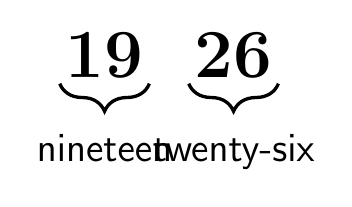
\begin{tikzpicture}[
            number/.style={
                font=\fontsize{60}{70}\selectfont\bfseries,
                inner sep=2pt,
                anchor=south west
            },
            label/.style={
                font=\Large\sffamily,
                anchor=north % 文字の上側を基準点にする
            },
            brace/.style={
                decorate,
                decoration={brace, amplitude=10pt, mirror},
                very thick
            }
        ]

            % --- Slide 1: 数字を表示 (<1-> 1枚目からずっと表示) ---
            
            \node<1->[number] (nineteen) at (0,0) {19};
            \node<1->[number, right=0.5cm of nineteen] (twentysix) {26};


            % --- Slide 2: 波かっこを表示 (<2-> 2枚目以降で表示) ---
            
            % 英語テキストと分離するため、ここでは draw コマンドのみにします
            \draw<2->[brace] (nineteen.south west) -- (nineteen.south east);
            \draw<2->[brace] (twentysix.south west) -- (twentysix.south east);


            % --- Slide 3: 英語を表示 (<3-> 3枚目以降で表示) ---
            
            % 波かっことは別のノードとして配置します。
            % 位置は「数字の下端(south)」から少し下(yshift)にずらした場所です。
            % 波かっこの深さ(10pt)より少し下になるように -15pt しています。
            
            \node<3->[label] at ([yshift=-15pt]nineteen.south) {nineteen};
            \node<3->[label] at ([yshift=-15pt]twentysix.south) {twenty-six};

        \end{tikzpicture}
    \end{overlayarea}
\end{frame}
%%%%%%%%%%%%%%%%%%%%%%%%%%%%%%%%%%%%%%%%%%%%%%%%%
\begin{frame}[plain]{Exercises}
 つぎの年号を英語で書きましょう

\visible<4->{yy00年~yy09年まではちょっぴり要注意}

\Large
\begin{enumerate}
 \item 1776\hfill\visible<2->{\makebox[80pt][l]{seventeen seventy-six}}\hspace{200pt}\mbox{}
 \item 1861\hfill\visible<3->{\makebox[80pt][l]{eighteen sixty-one}}\hspace{200pt}\mbox{}
 \item 1900\hfill\visible<5->{\makebox[80pt][l]{nineteen hundred}}\hspace{200pt}\mbox{}
 \item 1905\hfill\visible<6->{\makebox[80pt][l]{nineteen oh five}}\hspace{200pt}\mbox{}
 \item 1910\hfill\visible<7->{\makebox[80pt][l]{nineteen ten}}\hspace{200pt}\mbox{}
 \item 1998\hfill\visible<8->{\makebox[80pt][l]{nineteen ninety-eight}}\hspace{200pt}\mbox{}
\end{enumerate}

\mbox{}\hfill{\tiny 0244}\,{\scriptsize \myaudio{../1st_grader/audio/014_when_11.mp3}}

\end{frame}
%%%%%%%%%%%%%%%%%%%%%%%%%%%%%%%%%%%%%%%%%%%%%%%
\begin{frame}[plain]{Exercises}
\visible<3->{ややこしいのは2000年以降}

\Large
\begin{enumerate}
 \item 1999\hfill\visible<2->{\makebox[80pt][l]{nineteen ninety-nine}}\hspace{200pt}\mbox{}
 \item 2000\hfill\visible<4->{\makebox[80pt][l]{two thousand}}\hspace{200pt}\mbox{}
 \item 2003\hfill\visible<5->{\makebox[80pt][l]{two thousand three}}\hspace{200pt}\mbox{}
 \item 2009\hfill\visible<6->{\makebox[80pt][l]{two thousand nine}}\hspace{200pt}\mbox{}
 \item 2010\hfill\visible<7->{\makebox[80pt][l]{twenty ten\hspace{53.75pt}{\small (two thousand ten)}}}\hspace{200pt}\mbox{}
 \item 2020\hfill\visible<8->{\makebox[80pt][l]{twenty twenty\hspace{31.75pt}{\small (two thousand twenty)}}}\hspace{200pt}\mbox{}
 \item 2026\hfill\visible<9->{\makebox[80pt][l]{twenty twenty-six\hspace{5pt} {\small (two thousand twenty-six)}}}\hspace{200pt}\mbox{}
\end{enumerate}
\mbox{}\hfill{\tiny 0345}\,{\scriptsize \myaudio{../1st_grader/audio/014_when_12.mp3}}

\end{frame}
%%%%%%%%%%%%%%%%%%%
\begin{frame}[plain]{yyyy年mm月dd日}

\begin{description}[         ]
 \item[2026年2月5日] February 5, 2026 / February 5th, 2026\\
February (the) fifth, twenty twenty-six
\end{description}
\end{frame}
%%%%%%%%%%%%%%%%%%
\begin{frame}[plain]{My birthday is \fbox{      }}
 自分の誕生日(西暦yyyy年mm月dd日)を英語と数字で書いてみましょう。\\
また、その読み方を英語で書いてみましょう 

\vspace{80pt}
例:February 5, 2012 /  February 5th, 2012\\
\hfill(読み方February fifth, twenty twelve / two thousand twelve)
 
\end{frame}
%%%%%%%%%%%%%%%%%%%%%%%%%%%%%%%
%%%%%%%%%%%%%%%%%%%%%%%%%%%%%%%
\begin{frame}[plain]
 
\includegraphics[width=1.01\textwidth]{./infographic/002_day_month_season_infographic.png}
\end{frame}
%%%%%%%%%%%%%%%%%%%
%%%%%%%%%%%%%%%%%%%%%%%%%%%%%%%%%%%%%%
\begin{frame}[plain]
 
\hfill{\tiny audio\_overview 1139}\,{\scriptsize \myaudio{./audio/overview/002_day_month_season_audio_overview.m4a}}
\end{frame}
%%%%%%%%%%%%%%%%%%
\end{document}
